\documentclass[conference]{IEEEtran}
\IEEEoverridecommandlockouts
% The preceding line is only needed to identify funding in the first footnote. If that is unneeded, please comment it out.
\usepackage{cite}
\usepackage{amsmath,amssymb,amsfonts}
\usepackage{algorithmic}
\usepackage{graphicx}
\usepackage{textcomp}
\usepackage{xcolor}
\usepackage{amsfonts}
\usepackage{subcaption}
\usepackage{multirow}
\usepackage{makecell}
\usepackage{array}
\usepackage{booktabs}
\usepackage[backend=biber,style=ieee]{biblatex}
\addbibresource{ReferenceList.bib}
\usepackage{stfloats} % 用于跨列浮动环境
\def\BibTeX{{\rm B\kern-.05em{\sc i\kern-.025em b}\kern-.08em
    T\kern-.1667em\lower.7ex\hbox{E}\kern-.125emX}}
\begin{document}

\title{COMP 9517 Group Project Report\\
{\footnotesize \textsuperscript{}Team Tree New Bee: Riley Liu, Ruiqi Diao, Shilong Li (z5339228), Zhenlong An (Z5223659), Zhenyang Deng (z5407957)}
}

\maketitle

% \begin{abstract}
% This document is a model and instructions for \LaTeX.
% This and the IEEEtran.cls file define the components of your paper [title, text, heads, etc.]. *CRITICAL: Do Not Use Symbols, Special Characters, Footnotes, 
% or Math in Paper Title or Abstract.
% \end{abstract}

% \begin{IEEEkeywords}
% component, formatting, style, styling, insert
% \end{IEEEkeywords}

\section{Introduction}
Segmentation of individual sea turtles in marine environments represents a critical challenge in wildlife monitoring and conservation biology. While manual analysis has been the traditional approach, the exponential growth in photographic data—exemplified by the SeaTurtleID2022 dataset containing over 8,000 photographs of 438 individual sea turtles spanning 13 years—necessitates automated computer vision solutions. This research evaluates three state-of-the-art deep learning architectures—ResUNet++, DeeplabV3, and Mask R-CNN for semantic segmentation and instance segmentation of sea turtle anatomical features, specifically the head, flippers, and carapace. These architectures incorporate advanced mechanisms including attention gates and residual learning to address key challenges such as varying underwater lighting conditions, occlusions, and class imbalance in anatomical features. To enhance model performance, we implement a combined loss function incorporating class-weighted components, specifically designed to handle the inherent imbalance in feature representation. The study employs Intersection over Union (IoU) as the primary metric for performance evaluation, contributing to both computer vision advancement and ecological conservation efforts through robust, automated identification methodologies.
\section{Literature review}
\subsection{U-Net}
\subsubsection{Introduction of U-Net}
Ronneberger, Fischer and Brox [1] developed a convolutional network named U-Net, which comprise a contracting path and a symmetric expanding path enabling this network to capture context and precise localization. Moreover, U-Net require few images to train end-to-end and the calculating speed for this architecture is very fast. It can segment a 512x512 image within a second on a up to data GPU
\begin{figure}[h]
    \centering
    \begin{subfigure}[t]{0.23\textwidth}
        \centering
        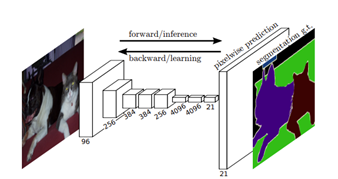
\includegraphics[width=\textwidth]{group/Picture1.png}
    \end{subfigure}%
    \hfill
    \begin{subfigure}[t]{0.23\textwidth}
        \centering
        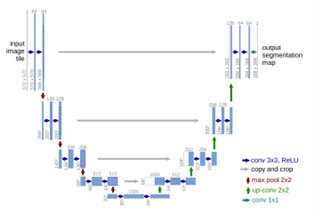
\includegraphics[width=\textwidth]{group/Picture2.png}
    \end{subfigure}
    \caption{(a) Fully convolutional network [2]. (b) U-Net architecture [1].}
\end{figure}
\textbf{Network Architecture}: The network architecture is illustrated in Figure 1 (b). The whole network formed by two parts, the contracting path (left side) and expansive path (right side). A typical convolutional network is followed by the contracting path. The contracting path includes a repeated implementation of two 3x3 convolutions (unpadded convolutions), each accompanied by a rectified linear unit (ReLU) and a 2x2 max pooling operation downsampling for 2 strides. For each downsampling step, this architecture replicates the number of feature channels. Each step in the expansive path comprises upsampling the feature map, followed by a 2x2 convolution (“up-convolution”) that splits the number of feature channels into two parts. This is then linked with the correspondingly cropped feature map from the contracting path followed by two 3x3 convolutions, each accompanied by a ReLU activation. The last final layer is a 1x1 convolution mapping each 64-component feature vector to the number of requested categories. There are 23 convolution layers in this structure.

\textbf{Mechanism}: The U-Net architecture consisting of a contracting path and an expansive path developed from the so-called “fully convolutional network” [2] (see Figure 1 a). Boosting a usual contracting network by successive layers is the basic concept in fully convolutional network [2], which the upsampling operators substitute the pooling operators. Therefore, these successive layers enhance the output resolution. In order to achieve the function of localization, the upsampled output ally with the high-resolution features generated from the contracting path. A more accurate output based on the information above can be assembled by the successive convolution layer.
One significant modification in the U-Net architecture is that the upsampling part contains a huge quantities of feature channels, empowering the higher resolution layers to capture context information. As a result, the expansive path is approximately symmetric to the contracting path, structuring a u-shaped network. Besides, the U-Net architecture only uses the valid part of each convolution, which means that it does not contain any fully connected layers. The scheme provides an overlap-tile strategy for seamless segmentation of any large images. 

One significant modification in the U-Net architecture is that the upsampling part contains a huge quantities of feature channels, empowering the higher resolution layers to capture context information. As a result, the expansive path is approximately symmetric to the contracting path, structuring a u-shaped network. Besides, the U-Net architecture only uses the valid part of each convolution, which means that it does not contain any fully connected layers. The scheme provides an overlap-tile strategy for seamless segmentation of any large images

\subsection{DeeplabV3}
Semantic segmentation, aimed at assigning semantic labels to every pixel in an image, is one of the fundamental topics in computer vision [14]. The encoder-decoder network has been successfully applied to numerous computer vision tasks, including object detection [12] and semantic segmentation [11]. Typically, the encoder-decoder network consists of two components: an encoder module that gradually reduces the feature maps and captures higher-level semantic information, and a decoder module that gradually recovers spatial information. The autoencoder model fully adheres to this concept [15], while U-Net incorporates skip connections between three encoders and decoders to effectively obtain sharper segmentation.

\subsubsection{Depthwise Separable Convolution}
Depthwise separable convolution or group convolution serves as a powerful operation to reduce both computation costs and the number of parameters while maintaining comparable performance [19]. This operation has been adopted in many recent neural network designs, such as flattened convolutional neural networks and the Xception model[17], showing improvements in both accuracy and speed for the task of semantic segmentation.

\subsubsection{Deep Convolutional Neural Networks and the DeepLab Series}
Deep convolutional neural networks based on Fully Convolutional Networks (FCNs) demonstrate significant improvements over systems relying on hand-crafted features in benchmark tasks [18]. DeepLabv3 utilizes several parallel atrous convolutions with different rates, known as Atrous Spatial Pyramid Pooling (ASPP)[19]. However, due to the design of state-of-the-art neural networks and limited GPU memory, it becomes computationally prohibitive to extract output feature maps that are 8 or 4 times smaller than the input resolution. The DeepLabv3+ model extends DeepLabv3 by adding an effective decoder module to recover object boundaries, allowing for detailed recovery of object contours [11].
\subsubsection{Long-Range Context Modeling}
One approach to enhancing the ability of convolutional neural networks (CNNs) to model long-range dependencies is through the adoption of self-attention [21] or non-local modules [20]. However, these methods notoriously consume vast memory resources to compute the large affinity matrix at each spatial position. Other strategies for long-range context modeling include dilated convolutions [22], which aim to widen the receptive field of CNNs without introducing additional parameters. A common limitation of these methods, including dilated convolutions and pooling, is that they probe input feature maps within square windows. Qinbin proposed a strip pooling module that narrows the pooling window [25], allowing the model to collect rich global contextual information and increase the receptive field of the backbone network; he also presented a mixed pooling module based on the classic residual block with a bottleneck structure.
\subsubsection{Residual Networks and Their Variants}
Furthermore, Targ et al. proposed a novel residual architecture known as ResNet-in-ResNet (RiR)[24], which incorporates residual blocks within the framework of a ResNet. The advantage of this model is the optimization benefits stemming from skip connections; however, the implementation requires tuning of additional parameters. Recent studies have also supported the notion that deep residual networks function akin to ensembles of relatively shallow networks [26], revealing the existence of exponential paths from the output layer to the input layer that gradient information can follow. Masoud introduced multi-residual networks that increase the multiplicity of the network while keeping its depth fixed[23].
Therefore, employing DeepLabv3+ for image segmentation can provide numerous advantages in terms of performance and cost-effectiveness. Strip pooling is lightweight and can serve as an efficient plug-and-play module for existing segmentation models. Multi-residual networks enhance the number of residual functions within the residual blocks, resulting in networks that are wider rather than deeper, thereby facilitating parallelism to reduce the computational cost of the network. Hence, we propose an improved DeepLabv3+ model that integrates strip pooling and multi-residual layers, which can offer numerous benefits in terms of efficiency and robustness, making it a promising option for a wide range of applications.
\subsection{Mask R-CNN}
Mask R-CNN first passes a feature map generated by ResNet50 and FPN to the Region Proposal Network (RPN) [10], applies a sliding window across the feature map, and uses pre-defined anchor boxes to generate potential object bounding boxes that possibly contain objects. In contrast to RoIPool, which reduces proposed regions to a consistent size via quantisation in Fast R-CNN, mask R-CNN introduces RoIAlign, a pixel-to-pixel alignment mechanism as mask predictions require more accurate and precise spatial features. [27] Extracted features will be passed through a pre-trained convolutional neural network. For each region of interest, a set of bounding boxes and class labels are predicted independent of pixel-wise masks as mask prediction will occur in parallel in the new branch of Mask R-CNN. Mask R-CNN is an extension of Fast R-CNN, originally used for object detection and will only generate bounding boxes and identify object classes. The key improvements from Fast R-CNN to Mask R-CNN [27] are applying a mask branch for instance segmentation, introducing RoI Align to preserve pixel accuracy and adopting a multi-task loss function that combines loss of classification, segmentation and position. These improvements allow Mask R-CNN to perform well in instance segmentation tasks and lay out the foundation of application on our dataset.
\section{Method}
To explore this project, we implemented different models based on U-Net and DeeplabV3 architecture. Our group compared the performance of two groups of network, the first group are U-Net, Attention U-Net and ResUNet++, the second group are different architecture in DeeplabV3+. In addition, we chose one theoretical different model, the Mask R-CNN, to evaluate the precision of fully convolutional encoder-decoder strategy and instance segmentation strategy.
\subsection{U-Net with Attention Gate and Deep Residual Learning}
\subsubsection{Attention (machine learning)}
Attention is a machine learning method for attending to an input vector’s different parts to catch long-term dependencies. According to the background of 
\begin{figure}[h]
    \centering
    \begin{subfigure}[t]{0.5\textwidth}
        \centering
        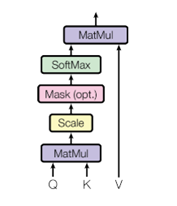
\includegraphics[width=0.4\textwidth]{group/Picture3.png}
    \end{subfigure}%
    \caption{Scaled Dot-Product Attention}
\end{figure}
Natural Language Processing (NLP), standard sequence-to-sequence models squeezed the input sequence to a fixed-length context vector, which obstructed their capability to remember long inputs, for example, sentences. On the other hand, attention produces shortcuts between the context vector and the entire source input [3].
\subsubsection{Attention Gate}
Attention Gate (AG) [5] is a variant of Attention mechanism concentrates on targeted regions while repressing feature activations in unrelated regions.
\begin{figure}[h]
    \centering
    \begin{subfigure}[t]{0.5\textwidth}
        \centering
        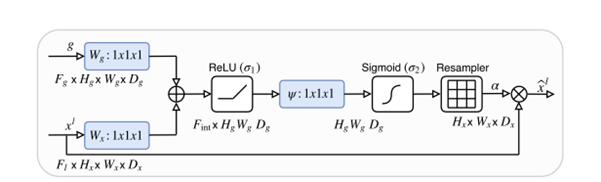
\includegraphics[width=\textwidth]{group/Picture4.png}
    \end{subfigure}%
    \caption{Scaled Dot-Product Attention}
\end{figure}
Given the input feature map $X$ and the gating signal $G\in\mathbb{R}^{C'\times H\times W}$ which is collected at a broad scale and holds contains contextual information, the attention gate utilizes additive attention to acquire the gating coefficient. Both the gating signal and the input $X$ are initially mapped linearly to an $\mathbb{R}^{F\times H \times W}$ dimensional space, after that, a spatial attention weight map $S\in\mathbb{R}^{1\times H\times W}$ is generated by compressing the output in the channel domain.
The overall process can be written as:
\begin{gather*}
    S=\sigma(\phi(\delta(\Phi_x(X)+\Phi_g (G))))\\
    Y=SX
\end{gather*}
Where $\phi$, $\Phi_x$ and $\Phi_g$ are linear transformations implemented as 1 × 1 convolution
\subsubsection{Residual Learning}
Residual Neural Network, also known as Residual Network or ResNet, is a deep learning architecture that the weight layers learn residual functions with reference to the layer inputs. One of the most important terminologies named “residual connection” refers to the specific architectural motif of $x\mapsto f(x)+x$ , in which $f$ is an arbitrary neural network module [4].
\subsubsection{Deep Residual U-Net}
Deep Residual U-Net, also called as Deep ResUNet. It is a semantic segmentation neural network build with residual units and has similar architecture of U-Net [6].
\begin{figure}[h]
    \centering
    \begin{subfigure}[t]{0.4\textwidth}
        \centering
        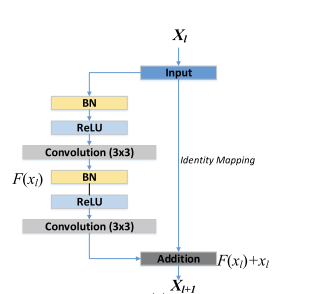
\includegraphics[width=0.7\textwidth]{group/Picture5.png}
    \end{subfigure}%
    \caption{Residual unit with identity mapping used in the ResUnet [6].}
\end{figure}
The residual neural network includes a number of stacked residual units. The residual unit can be described as a form:
\begin{gather*}
    y_l=h(x_l)+F(x_l,w_l)\\
    x_(l+1)=f(y_l)
\end{gather*} 
where $x_l$ and $x_{(l+1)}$ are the input and output of the $l$th residual unit $F$, $f$ and $h$ are the residual function, activation function and identity mapping function respectively.


Through the residual unit, Zhengxin et al.(2018) [6] built a deep ResUnet architecture as shown in Fig. 5. This network structure combines two benefits 
\begin{figure}[h]
    \centering
    \begin{subfigure}[t]{0.2\textwidth}
        \centering
        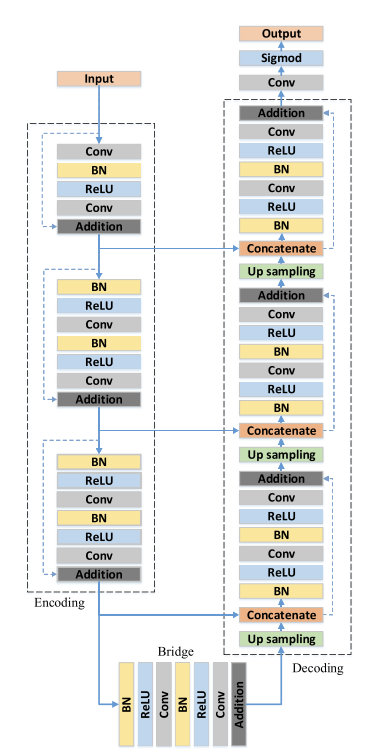
\includegraphics[width=\textwidth]{group/Picture6.png}
    \end{subfigure}%
    \hfill
    \begin{subfigure}[t]{0.26\textwidth}
        \centering
        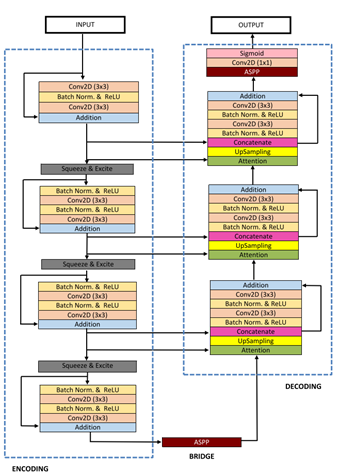
\includegraphics[width=\textwidth]{group/Picture7.png}
    \end{subfigure}%
    \caption{Architecture of deep ResUnet[6] (Left), and Architecture of ResUNet++[7] (Right)}
\end{figure}
From different aspects. First, the residual unit allows an ease training of this network. Second, the residual unit combined with the skip connections between low levels and high levels of the network will assist information propagation without degradation. Which brings us a possibility to develop a neural network with a significant fewer parameters.
\subsubsection{ResUNet++}
Based on the information above, Debesh et al. (2019) [7] raised a segmentation architecture that utilizes the advantage of deep residual learning and attention gate with U-Net.
\subsection{DeeplabV3+}
\subsubsection{Segmentation Network}
Previous studies have demonstrated that DeepLabV3+ can achieve remarkable segmentation results [11]. Therefore, it is optimized in this study as the benchmark model for turtle segmentation. The block diagram of the DeeplabV3 plus segmentation model is illustrated in Figure 6. The model comprises two main components: an encoder and a decoder.
To effectively extract features of turtles from the given images, the encoder includes a backbone network and an improved Atrous Spatial Pyramid Pooling (ASPP). The backbone network utilizes ResNet101. We propose an improved ASPP performs parallel operations of improved multi-residual atrous convolution with varying dilation rates and enhanced strip pooling, instead of regular atrous convolution and global average pooling. Specifically, three 3x3 convolutions are performed with dilation rates of 6, 12, and 18, respectively. These variations expand the receptive field and improve localization detection accuracy without losing resolution. This operation condenses the features extracted by the improved backbone network into multi-scale contextual semantic information. 
In the decoder, the output features of the encoder are first bilinearly upsampled by a factor of 4, followed by a concatenation with the low-level features from the improved backbone in the channel dimension. To reduce the number of channels in the low-level features, a 1x1 convolution is applied prior to concatenation, followed by a 3x3 convolution operation to refine the features. Finally, a bilinear upsampling operation by a factor of 4 is performed to yield the final semantic segmentation results.
\begin{figure}[h]
    \centering
    \begin{subfigure}[t]{0.4\textwidth}
        \centering
        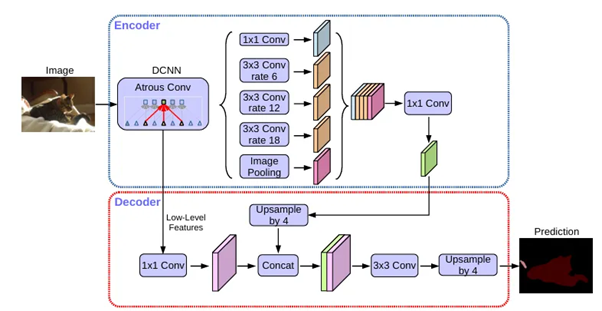
\includegraphics[width=\textwidth]{group/Picture8.png}
    \end{subfigure}%
    \caption{Architecture of DeeplabV3 segmentation network [11]}
\end{figure}
\subsubsection{Improved multi-residual atrous convolution}
The improved multi-residual atrous convolution integrates two multi scale residual blocks while introducing dilation to preserve the features of atrous convolution [23]. This approach provides several benefits, including enhanced feature extraction, minimized overfitting, superior resolution adaptability, a wider network structure, and improved handling of class imbalances. By utilizing two parallel multi scale dilated residual blocks with varying scale parameters, dual multi scale residual blocks can capture a broader range of features across different input image scales, resulting in diverse and complementary feature learning. The parallel arrangement of dual multi scale residual blocks also promotes gradient flow during back-propagation as illustrated in Figure 7, thereby aiding in training deeper networks and alleviating the vanishing gradient issue. Overall, dual multi scale residual with dilated ratio blocks present a robust and efficient methodology for image segmentation tasks by leveraging multiple scales, expanding the receptive field and refined feature extraction. 
\begin{figure}[h]
    \centering
    \begin{subfigure}[t]{0.4\textwidth}
        \centering
        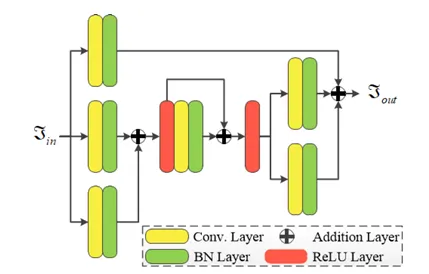
\includegraphics[width=\textwidth]{group/Picture9.png}
    \end{subfigure}%
    \caption{Improved multi-residual atrous convolution [18]}
\end{figure}
\subsubsection{Strip Pooling Module}
The Strip Pooling Module leverages both horizontal and vertical strip pooling operations to capture long-range context from various spatial dimensions [15]. Initially, the input tensor x is fed into two parallel pathways, each containing either a horizontal or vertical strip pooling layer followed by a 1D convolutional layer with a kernel size of 3, which modulates the current location and its neighboring features.
During this process, each position in the output tensor can establish relationships with a variety of positions in the input tensor. For example, as illustrated in Figure 8, the square bounded by the black box in the output tensor is connected to all locations that share the same horizontal or vertical coordinates (enclosed by the red and purple boxes). Therefore, by repeating the above aggregation process multiple times, it becomes possible to build long-range dependencies across the entire scene. Moreover, benefiting from the element-wise multiplication operation, the proposed Strip Pooling Module can also be considered an attention mechanism and can be directly applied to any pretrained backbone networks without the need to retrain them from scratch [15].
\begin{figure}[h]
    \centering
    \begin{subfigure}[t]{0.4\textwidth}
        \centering
        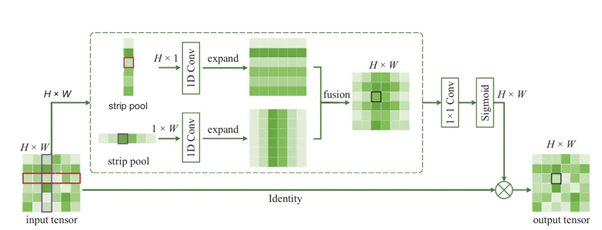
\includegraphics[width=\textwidth]{group/Picture10.png}
    \end{subfigure}%
    \caption{Schematic illustration of the Strip Pooling module [15]}
\end{figure}
\subsection{Mask R-CNN}
Mask R-CNN was chosen due to its effectiveness in mask prediction and its novel application of instance segmentation techniques to instance segmentation tasks. Mask R-CNN achieves state-of-the-art performance in instance segmentation, making it a strong candidate for tasks requiring accurate mask localization. While models like U-Net [28] and DeepLabv3 [29] are often used directly for semantic segmentation, applying Mask R-CNN leverages its robust instance segmentation capabilities creatively. The use of a multi-task loss function [27] also enhances mask prediction accuracy by allowing better localization. 
The Mask R-CNN model uses ResNet50 with a Feature Pyramid Network (FPN) [30] as its backbone, initialized with pre-trained weights. The FastRCNNPredictor and MaskRCNNPredictor heads are modified to adapt four output classes: background, carapace, flipper, and head. Experimental dropout is applied after the linear layers in the box prediction head to prevent overfitting, as the model tends to converge quickly
\begin{figure}[h]
    \centering
    \begin{subfigure}[t]{0.4\textwidth}
        \centering
        \includegraphics[width=\textwidth]{group/Picture11.png}
    \end{subfigure}%
    \caption{The Mask R-CNN structure for object detection and instance segmentation tasks [31]}
\end{figure}
\subsection{Preparing the Dataset}
In this study, we utilize the image dataset from SeaTurtleID2022, which contains a total of 438 individual sea turtles. To enhance the robustness and enrich our dataset, we employed several augmentation strategies, including random rotation, random cropping, random brightness and contrast adjustments, random blurring, and noise addition, among others. Image preprocessing was performed to reduce computational costs and improve efficiency. All images were uniformly resized to 1024 x 1024 pixels. The dataset used in this research was divided into training, validation, and testing subsets according to an open-set splitting file. This open-set splitting provides a significant increase on realistic performance evaluation compared to random splitting or closed-set splitting [8]. 
\subsection{Loss Function}
In this study, we observed that the head and legs have a significantly smaller number of pixels compared to the background. The carapace, while larger than the head and legs, is still smaller than the background. The frequency differences among the four categories can cause an imbalance during training, which may lead to the underestimation of the importance of target pixels. Therefore, a combined loss function was employed in this study, consisting of class-weighted Dice loss, class-weighted focal loss, and class-weighted cross-entropy loss. The final weights assigned to the dataset are 0.02 for the head, 0.21 for the legs, 0.63 for the carapace, and 1.0 for the background.

Class-weighted Dice loss is particularly effective in addressing imbalances in class distribution. It measures the overlap between the predicted and ground truth segmentation, emphasizing the importance of smaller classes by weighting them differently. This is beneficial in cases where certain classes (like the head and legs) are underrepresented.
Class-weighted focal loss is designed to address the issue of class imbalance by focusing more on hard-to-classify examples. It consists of a modulating factor that reduces the relative loss for well-classified examples, putting more focus on challenging cases. This property is especially useful in tasks involving high variability in class frequencies, helping the model better learn from those difficult instances.
Class-weighted cross-entropy loss is a widely used loss function in classification tasks. By applying class weights, it allows the model to give more importance to less frequent classes while still ensuring a standard probabilistic interpretation of the predicted classifications. This can help achieve a balanced learning process across all classes.
The weights are calculated using the following formula:
$$
W_m=\mathbf{N}(\frac{mean fre}{fre_m })
$$
where $fre_m$ represents the frequency of occurrences of pixels in class mm divided by the total number of pixels in any image containing that class and mean $fre$  denotes the mean of these frequencies across each image. $\mathbf{N}$ is the normalization factor for all weights. Therefore, the overall loss function is formulated as:
$$
loss=p\times dice+q\times focal+z\times cross
$$
where $dice$ is the Dice loss, $focal$ is the focal loss, and $cross$ is the cross-entropy loss. The constants $p,q,z$ are used to balance the contributions of the three loss components.

\subsection{Implementation Details}
All architectures were implemented using the TensorFlow frame [9]. We performed our experiment on a single GPU RTX A6000 (NVIDIA). The training system is part of Additive Manufacturing Laboratories heterogeneous cluster and has an Intel(R) 13th Gen Core (TM) i9-13900K CPU 3.00 GHz, 128G of DDR4-2667MHz DRAM. We start the training with a batch size of 8, and the proposed architectures are optimized by Adam optimizer. We set a learning rate adjustment schedule with 1e-4 as the beginning rate. This schedule will increase the learning rate to 1e-3 empowering models to have a better learning outcome. After this model reached the max learning rate, the schedule will decrease it on the later part of the training to prevent over-fitting.
\section{Experimental Results}
After training, the results show that ResUNet++ achieved a boosted performance for the “SeaTurtleID2022” dataset comparing to U-Net and Attention U-Net. Specifically data see table 1.

\begin{table*}[!t]
\centering
\renewcommand{\arraystretch}{1.3} % 调整行高
\setlength{\tabcolsep}{3pt} % 调整列间距
\caption{Performance Comparison of Different Models}
\begin{tabular}{|c|c|c|c|c|c|c|c|c|c|c|c|c|c|}
\hline
\multirow{2}{*}{Model} & \multirow{2}{*}{Loss} & \multicolumn{4}{c|}{IoU} & \multicolumn{4}{c|}{Recall} & \multicolumn{4}{c|}{Precision} \\ \cline{3-14} 
 &  & Turtle & Legs & Head & Overall & Turtle & Legs & Head & Overall & Turtle & Legs & Head & Overall \\ \hline
U-Net & 0.0683 & 0.8694 & \textbf{0.8254} & 0.8339 & 0.8794 & 0.9362 & \textbf{0.8953} & 0.8866 & 0.9284 & 0.9214 & 0.9112 & 0.9364 & 0.9405 \\ \hline
Attention U-Net & 0.0601 & 0.8722 & 0.8153 & 0.8423 & 0.8811 & 0.9413 & 0.8901 & 0.8911 & 0.9302 & 0.9279 & 0.9133 & 0.9383 & 0.9443 \\ \hline
ResUNet++ & \textbf{0.0483} & \textbf{0.8927} & 0.8157 & \textbf{0.8603} & \textbf{0.8899} & \textbf{0.9494} & 0.8800 & \textbf{0.9065} & \textbf{0.9333} & \textbf{0.9355} & \textbf{0.9159} & \textbf{0.9468} & \textbf{0.9479} \\ \hline
\hline
DeepLabV3-baseline & \textbf{0.1500} & \textbf{0.9431} & 0.8495 & 0.9203 & 0.9270 & 0.9716 & \textbf{0.9804} & 0.9832 & \textbf{0.9828} & \textbf{0.9697} & 0.8636 & 0.9350 & 0.9418 \\ \hline
DeepLabV3 + Strip Pooling & 0.1501 & 0.9422 & \textbf{0.8521} & 0.9098 & 0.9248 & 0.9740 & 0.9747 & \textbf{0.9845} & 0.9822 & 0.9663 & 0.8637 & 0.9231 & 0.9398 \\ \hline
DeepLabV3 + multi-residual & 0.1501 & 0.9427 & 0.8478 & 0.9148 & 0.9251 & 0.9735 & 0.9748 & 0.9841 & 0.9821 & 0.9675 & \textbf{0.8708} & 0.9286 & 0.9404 \\ \hline
DeepLabV3 + SP + MR & 0.1501 & 0.9421 & 0.8486 & \textbf{0.9245} & \textbf{0.9275} & \textbf{0.9754} & 0.9757 & 0.9827 & 0.9824 & 0.9649 & 0.8666 & \textbf{0.9398} & \textbf{0.9426} \\ \hline
\hline
Mask R-Cnn & 0.3613 & 0.9276 & 0.7807 & 0.8051 & 0.8378 & 0.9317 & 0.7911 & 0.7997 & 0.8433 & 0.9211 & 0.7907 & 0.8071 & 0.8213 \\ \hline
\end{tabular}
\end{table*}
Based on table 1, we found that the performance of ResUNet++ is generally better than the other two basic networks. Benefitting from the residual connections, ResUNet++ could pass feature information and make it easier for models to learn identity mappings. Thus, the result of ResUNet++ is a little bit competent than basic UNet structure. Attention mechanism is also worked in this group.

In addition to compare data between the same theoretical architecture. Our group also trained DeeplabV3 and Mask R-CNN which have a totally different logic in structure design.

We have applied different combinations of hyperparameters, for example, the learning rate, number of epochs, batch size, filter size and the optimizer, to optimize our ResUNet++ architecture. Our team manually trained the models with different group of values and evaluated their results. Table 1 presents the final performance value of ResUNet++ with the highest mIoU and precision. The ResUNet++ architecture achieved the best performance through its powerful attention units and residual blocks. Besides, the DeepLabV3 models also fit this project well with high mIoU score, recall and precision.

Considering the IoU score of different parts of these models, DeeplabV3 architecture has the highest accuracy comparing to ResUNet and Mask R-CNN, especially in the legs and head part. One core feature of DeepLabV3 is the Atrous Spatial Pyramid Pooling (ASPP) module that utilizes multiple dilated convolution layers with different rates. Within the multi-scale feature extraction, DeepLabV3 is critical for small object segmenting. Thus, it is theoretically performed better than other two types of models. While ResUNet++ has a highly specialized encoder-decoder structure with residual block and skip connections. Which is mean that ResUNet is effective for large objects dominated segmentation tasks or when deep context is less critical

Mask R-CNN are designed with a larger receptive field, empowering them to learn broader contextual information. However, this theoretic different designed architecture can also cause them overlook or dilute smaller details. The structure of ResUNet++ helps it maintain a balanced understanding of global and local features. That is why Mask R-CNN is better at specific IoU score while other part is not competitive 

\begin{figure}[!t]
    \centering
    \begin{subfigure}[t]{0.23\textwidth}
        \centering
        \includegraphics[width=\textwidth]{deeplabv3_all_image_222.jpg}
        \caption{Image}
    \end{subfigure}
    \hfill
    \begin{subfigure}[t]{0.23\textwidth}
        \centering
        \includegraphics[width=\textwidth]{deeplabv3_all_mask_222.jpg}
        \caption{True Mask}
    \end{subfigure}
    \vspace{0.5em}
    \begin{subfigure}[t]{0.23\textwidth}
        \centering
        \includegraphics[width=\textwidth]{deeplabv3_all_pred_222.jpg}
        \caption{Pred (DeepLabV3+ SP + MR)}
    \end{subfigure}
    \hfill
    \begin{subfigure}[t]{0.23\textwidth}
        \centering
        \includegraphics[width=\textwidth]{pred_mask.png}
        \caption{Pred (ResUNet++)}
    \end{subfigure}

    \vspace{0.5em}
    \begin{subfigure}[t]{0.23\textwidth}
        \centering
        \includegraphics[width=\textwidth]{rcnn_pred.png}
        \caption{Pred (Mask R-CNN)}
    \end{subfigure}
    \hfill
    \begin{subfigure}[t]{0.23\textwidth}
        \centering
        \includegraphics[width=\textwidth]{rcnn_true.png}
        \caption{True Mask (Mask R-CNN)}
    \end{subfigure}

    \caption{Example segmentation result of three models. }
\end{figure}

\begin{table}[h]
\centering
\renewcommand{\arraystretch}{1.2} % Adjust row height
\setlength{\tabcolsep}{6pt} % Adjust column spacing
\caption{Performance Metrics of Different Models}
\begin{tabular}{|c|c|c|c|c|}
\hline
\textbf{Model} & \textbf{MIoU} & \textbf{Loss} & \textbf{Recall} & \textbf{Precision} \\ \hline
ResUNet++ & 0.8899 & \textbf{0.0483} & 0.9333 & \textbf{0.9479} \\ \hline
DeepLabV3+ & \textbf{0.9275} & 0.1501 & \textbf{0.9824} & 0.9426 \\ \hline
Mask R-CNN & 0.8378 & 0.3613 & 0.8433 & 0.8213 \\ \hline
\end{tabular}
\end{table}
\section{Discussion}
The sea turtle images segmented using the different methods implemented in this project underlined opportunities and constraints in the application of automated approaches to sea turtle identification and monitoring. In particular, deep learning-based models U-Net and Mask R-CNN proved efficient to segment essential parts of sea turtles: their heads, flippers, and the carapace (the upper section of the turtle's shell). A comparative study between these two methods indicated that though both perform exceptionally well under normal conditions, there lies a significant difference in terms of their robustness and adaptability in handling diversified challenging environmental factors comprising variation in illumination, underwater reflections, and occlusions.

To boost the performance of the models, their structure and parameters, on the one hand, and a new loss function, on the other hand, can be developed.

1) \textbf{Model Optimization (Structure and Parameters)}: Proper model structure and parameter fine-tuning would go a long way toward improving segmentation performance. For example, upgrading the U-Net architecture with more skip connections or attention mechanisms would ensure better generalization in difficult conditions. Adapting Mask R-CNN to alternative region proposal strategies, or having a more profound backbone network, may ensure much more progressive improvements regarding complex underwater scene understanding tasks. Further adjustments to hyperparameter configurations for several combinations of variations, such as learning rate schedules, batch sizes, and optimization algorithms, must be defined for the actual problem. Hybrid architectures, leveraging the power of both U-Net and Mask R-CNN, could also be the way forward to better segmentation results.

2) \textbf{New Loss Function}: A new loss function may be designed based on the problematics of segmentation for sea turtles, addressing the issue of class imbalance and overall improving model performance. The present use of IoU makes small things shine most where the models got stuck, such as flippers and head regions. A plausible alternative could be constituting a composite loss comprising class-weighted Dice loss with focal and cross-entropy losses to give more weight to ignored smaller regions. This would enable the models to learn better from challenging examples and ensure more accurate segmentation of smaller parts even when they are occluded or under poor lighting.

These optimization strategies could be studied in greater detail in future work. Furthermore, developing more advanced models like those based on Transformers would ensure the highest possible segmentation results, particularly when dealing with complexities and diversities in different underwater scenarios. Perhaps further enriching the dataset through synthetic generations or enhanced annotation techniques may be considered as paths to bolstering model strength and accuracy.
\section{Conclusion}
This research evaluated ResUNet++, DeeplabV3, and Mask R-CNN architectures - for sea turtle segmentation utilizing the SeaTurtleID2022 dataset. The findings reveal significant insights into the effectiveness of various approaches and highlight areas for future development in marine creature segmentation
\subsection{What worked successfully}
The multi-task loss function, combining class-weighted Dice loss, focal loss, and cross-entropy loss, effectively addressed class imbalance challenges. The weighting system (0.02 for head, 0.21 for legs, 0.63 for carapace, 1.0 for background) improved feature learning across anatomical structures, while the focal loss component enhanced performance on challenging examples.

DeeplabV3's strip pooling module captured long-range contextual information through horizontal and vertical operations. The multi-residual atrous convolution extracted features at multiple scales, handling varying turtle sizes and orientations. ResNet101 backbone with improved ASPP demonstrated robust feature extraction in underwater environments.

Mask R-CNN's RoIAlign mechanism achieved precise spatial alignment for accurate mask prediction. ResNet50 with FPN backbone handled multi-scale feature extraction, while parallel mask prediction successfully separated instance segmentation from classification tasks.
\subsection{What Did Not Work As Expected}
The standard U-Net architecture without attention mechanisms showed poor performance compared to our enhanced models. It struggled to segment small anatomical features like turtle heads and flippers, especially in complex underwater environments. The model frequently misclassified these features due to class imbalance and inadequate feature extraction capabilities, resulting in fragmented segmentation outputs.

The basic DeeplabV3 implementation, despite showing reasonable segmentation metrics, fell short compared to our enhanced version with strip pooling and multi-residual layers. It failed to handle varying underwater lighting conditions and struggled with long-range dependencies, leading to inconsistent segmentation results particularly when turtle features overlapped or were partially occluded.

The initial Mask R-CNN configuration, while providing precise instance segmentation, encountered significant computational limitations. The model required excessive GPU memory, limiting batch sizes to 8 on our RTX A6000 GPU, and struggled with real-time processing requirements. Additionally, the standard RoIPool operations resulted in misaligned feature maps, affecting the accuracy of boundary predictions in complex underwater scenes.
\subsection{Future improvement Section}

\textbf{Enhanced Multi-residual Learning:} Further improve DeeplabV3's performance by incorporating additional residual connections and adaptive feature fusion mechanisms. This enhancement would strengthen feature propagation and address the vanishing gradient problem, particularly beneficial for deep underwater feature extraction.

\textbf{Advanced Attention Integration:} Investigate applying sophisticated attention mechanisms like spatial-channel attention and strip-wise attention pooling across all three architectures. This would enhance the models' ability to focus on critical anatomical features while suppressing irrelevant underwater background noise

\textbf{Adaptive Loss Function Development:} Develop a dynamic weighting scheme for the multi-task loss function that automatically adjusts based on training progress and feature complexity. That would better address class imbalance issues and improve segmentation accuracy for smaller anatomical features.

\textbf{Underwater-Specific Data Augmentation:} Implement specialized augmentation techniques simulating various underwater conditions, including water turbidity, lighting variations, and refraction effects. This would enhance model robustness across diverse marine environments and improve generalization capabilities.

\textbf{Efficient Architecture Design:} Explore lightweight variants of our current architectures using techniques like network pruning and knowledge distillation. This would address computational constraints while maintaining segmentation accuracy, enabling real-time processing for practical marine biology applications.

\textbf{Multi-Modal Integration Framework:} Develop a comprehensive framework that combines RGB image data with additional modalities such as depth information and temporal sequences. This integration would provide richer feature representations and improve segmentation accuracy in challenging underwater scenarios, particularly for partially occluded turtle features.
 
By implementing these improvements, we can achieve more accurate and efficient sea turtle segmentation, directly supporting marine biologists in their conservation efforts and population monitoring tasks.
\small
\printbibliography
\nocite{*}
\normalsize
\end{document}

\newpage


\section*{Acknowledgment}

The preferred spelling of the word ``acknowledgment'' in America is without 
an ``e'' after the ``g''. Avoid the stilted expression ``one of us (R. B. 
G.) thanks $\ldots$''. Instead, try ``R. B. G. thanks$\ldots$''. Put sponsor 
acknowledgments in the unnumbered footnote on the first page.

\section*{References}

Please number citations consecutively within brackets \cite{b1}. The 
sentence punctuation follows the bracket \cite{b2}. Refer simply to the reference 
number, as in \cite{b3}---do not use ``Ref. \cite{b3}'' or ``reference \cite{b3}'' except at 
the beginning of a sentence: ``Reference \cite{b3} was the first $\ldots$''

Number footnotes separately in superscripts. Place the actual footnote at 
the bottom of the column in which it was cited. Do not put footnotes in the 
abstract or reference list. Use letters for table footnotes.

Unless there are six authors or more give all authors' names; do not use 
``et al.''. Papers that have not been published, even if they have been 
submitted for publication, should be cited as ``unpublished'' \cite{b4}. Papers 
that have been accepted for publication should be cited as ``in press'' \cite{b5}. 
Capitalize only the first word in a paper title, except for proper nouns and 
element symbols.

For papers published in translation journals, please give the English 
citation first, followed by the original foreign-language citation \cite{b6}.

\begin{thebibliography}{00}
\bibitem{b1} G. Eason, B. Noble, and I. N. Sneddon, ``On certain integrals of Lipschitz-Hankel type involving products of Bessel functions,'' Phil. Trans. Roy. Soc. London, vol. A247, pp. 529--551, April 1955.
\bibitem{b2} J. Clerk Maxwell, A Treatise on Electricity and Magnetism, 3rd ed., vol. 2. Oxford: Clarendon, 1892, pp.68--73.
\bibitem{b3} I. S. Jacobs and C. P. Bean, ``Fine particles, thin films and exchange anisotropy,'' in Magnetism, vol. III, G. T. Rado and H. Suhl, Eds. New York: Academic, 1963, pp. 271--350.
\bibitem{b4} K. Elissa, ``Title of paper if known,'' unpublished.
\bibitem{b5} R. Nicole, ``Title of paper with only first word capitalized,'' J. Name Stand. Abbrev., in press.
\bibitem{b6} Y. Yorozu, M. Hirano, K. Oka, and Y. Tagawa, ``Electron spectroscopy studies on magneto-optical media and plastic substrate interface,'' IEEE Transl. J. Magn. Japan, vol. 2, pp. 740--741, August 1987 [Digests 9th Annual Conf. Magnetics Japan, p. 301, 1982].
\bibitem{b7} M. Young, The Technical Writer's Handbook. Mill Valley, CA: University Science, 1989.
\end{thebibliography}
\vspace{12pt}
\color{red}
IEEE conference templates contain guidance text for composing and formatting conference papers. Please ensure that all template text is removed from your conference paper prior to submission to the conference. Failure to remove the template text from your paper may result in your paper not being published.

\end{document}
